%&electrodcheat
\documentclass{trchesh}
\usepackage{trmath}
\usepackage{trsym} 

\setlayout[page-orient=landscape, size=10]{hardcopy}
\makeatletter
\def\note{\ifexpmode{\@gobble}{\endnote}}
\makeatother
\usepackage{tikz}
\usepackage{pgfplots}
\pgfplotsset{compat=1.11}
\usetikzlibrary{external,calc,arrows}
\tikzsetexternalprefix{img/}
\tikzexternalize%
\usepackage{docmute}
\hypersetup{
  pdftitle={Шпора по электроду},
  pdfauthor={taxus},
  pdfsubject={Электродинамика},
  pdfkeywords={Электродинамика;СПбГУ;by-taxus}
}
\columnseprule=0.1dd
\def\arraystretch{1.3}
\setlist[enumerate,1]{leftmargin=1.6em}
\setlist[itemize,1]{leftmargin=2em, label=$\triangleright$}

\def\waveop{\mathop{\boldsymbol\Box}}

\newcommand{\deflabel}[1]{
  \makebox[\labelwidth][l]{%
    \parbox[t]{\labelwidth}{\hspace{0pt}\textsf{#1}}%
  }~::
}
\newenvironment{defs}[1][\hspace{12ex}]%
  {\begin{list}{}{%
        \let \makelabel=\deflabel%
        \setlength{\labelwidth}{\widthof{#1}} %
        \setlength{\leftmargin}{\labelwidth+\labelsep}%
        \itemsep=0pt %
      }}%
  {\end{list}}
\newenvironment{facts}{\begin{list}{$\triangleright$}{}}{\end{list}}

\graphicspath{{img/}}
\begin{document}
\begin{multicols*}{3}\raggedright%
\parindent=0pt
\paragraph{Уравнения Максвелла}
\begin{enumerate}
  \item Теорема Гаусса: $\oint \v E \cdot \del \v s = 4 \pi Q$.
  \item Закон Фарадея: $\oint\v E \cdot \del \v l = - \frac{1}{c} \pder{\Phi}{t}$, \\
    $\Phi=\int \v B \cdot \del \v s$
  \item Закон Био-Савара-Лапласа: $\v B = \frac{1}{c} \, \frac{\v j \times \v R}{R^3}$
  \item $\oint \v B \cdot \del \v s = 0$
  \item Закон Ампера: $\oint \v B \cdot \del \v l = \frac{4 \pi}{c} \int \v j \cdot \del \v s$
  \item Уравнение неразрывности: $\pder \rho t  + \div \v j = 0 $
  \item Сами уравения Максвелла: \par\vspace{1ex}$
    \begin{aligned}
      &\div \v E &&=&& 4 \pi \rho \\
      &\div \v B &&=&& 0 \\
      &\rot \v E &&=&& - \frac 1 c \, \pder{\v B}{t} \\
      &\rot \v B &&=&& \frac 1 c\, \pder{\v E}{t} + \frac{4 \pi}{c}\v j
    \end{aligned}$
\end{enumerate}

\paragraph{В среде}
\begin{enumerate}
  \item Поляризация и намагниченность \\
    $\begin{aligned}
    \v P \that\v j_{\mathrm{pol}} &=\pder{\v P}t,\;\rho_{\mathrm{pol}} =-\div \v P,\\
    \v M \that \v j_{\mathrm{m}} &= c \rot \v M \\
    \{\rho, \v j\}_{\mathrm{int}} &= \{\rho, \v j\}_{\mathrm{pol}} + \{\rho, \v j\}_{\mathrm{m}}
    \end{aligned}$
\item В сильнопеременных  \par
$
\begin{aligned}
  \rho_{\mathrm{int}} &= - \div \v P \\
  \v j_{\mathrm{int}} &= \pder{\v P}{t}  + c \rot \v M
\end{aligned}
$
\item $\v D = \v E + 4 \pi \v P$, $\v H = \v B - 4 \pi \v M$
\item Уравнения Максвелла в среде: \par
  $ \begin{aligned}
        \div \v D &= 4 \pi \rho_{ex} \\
        \rot \v H &= \frac 1 c \, \pder {\v D} t + \frac{4\pi}{c} \,
        (\v j_{ex} + \v j _{c})           
      \end{aligned}$
\item Материальные уравнения (простейшие)\par
  $\v D = \varepsilon \v E,\;\v B = \mu \v H ,\;\v j_c = \sigma \v E$
\item Дисперсия, варианты \par
  $ \begin{aligned}
    \v D (\v r,t) &= \int_{-\infty}^t f (t' - t, \v r)\,\v E(\v r, t')\, \del t \\
    \v D (\v r,t) &= \int_{\Delta V} g(\v r' -\v r, t)\,\v E(\v r, t')\, \del V
  \end{aligned} $ \par
$f,g$~--- функция отклика.
\end{enumerate}


\paragraph{Энергетические соотношения}
$
  \begin{aligned}
    w &= \frac{1}{8 \pi} \, (\varepsilon E^2 + \mu H^2) \\
    \v S &= \frac{c}{4 \pi} \, \v E \times \v H \\
    \pder{w}{t} + \div \v S &= - \sigma E^2 - \v E \cdot \v j_{ex}
  \end{aligned}
$ \par
Так что если внешние силы не совершают работы, 
энергия лишь убывает (за счёт выделения тепла).

\paragraph{Потенциал}
\begin{enumerate}
  \item Вид потенциала:
    $ \v E = - \frac 1 c \pder{\v A} t  - \nabla \varphi$,
    $\v B = \rot \v A$
  \item Калибровочная инвариантность:
    $ \left\{\begin{aligned}
      \v A' &= \v A - \nabla \chi \\
      \varphi' &= \varphi + \frac{1}{c} \, \pder{\chi}{t}
  \end{aligned}\right.$
  \item Калибровка  Лоренца: 
      $\frac{\varepsilon \mu}{c} \, \pder{\varphi}t + \div \v A = 0$%
      \note{при этом подходят все $\chi \that \waveop \chi = 0$}
    \item Уравнения Максвелла примут вид: 
      $
      \begin{aligned}
        \waveop \varphi &= \frac{4 \pi}{\varepsilon}\, \rho, \\
        \waveop \v A &= \frac{4 \pi \mu}{c} \, \v j, 
        \text{ где }\waveop = \frac{1}{v^2} \, \pder[2]{}{t} - \nabla,
        v = \frac{c}{\sqrt{\varepsilon \mu}} 
      \end{aligned}
      $
\end{enumerate}
\paragraph{Волновые уравнения}
$
\begin{aligned}
\waveop \v E = 0, \; \waveop \v B  =0 \\
\waveop \v A =0, \; \waveop \varphi  =0  \qquad (\waveop \chi = 0 )
\end{aligned}
$

Ещё можно $\varphi$ занулить, выбрав нужную $\chi$
\note{В предыдущем нельзя, может не оказаться решением}

\paragraph{Плоские и сферические волны}
\begin{enumerate}
  \item Одномерное волновое уравнение и его решение:
    $
    \begin{aligned}
    \frac 1 {v^2} \, \pder[2]{u}{t} - \pder[2]{u}{x} = 0 \\
    u = f(x-vt) + g(x+vt)
    \end{aligned}
    $
  \item Плоская волна: $A =  A(\v n \cdot \v r - vt)$ \note{вторую волну выкинули,
    нам обычно хватает какого-то частного решения.}
  \item Условие поперечности: $\div \v A = 0$ $\Rightarrow$ $\v B = \frac cv \,\v n \times \v E$ 
  \item $\v S = v \, w \, \v n$.
  \item Уравнение сферической волны: $\frac{1}{v^2}\,\pder[2]{u}{t} - \Delta_r u = 0$
  \item Его решение: $u(r,t) = \frac{1}{r}\bigl(f(r-vt) + g(r+vt)\bigr) $
    Если рассматривать монохроматические волны, произвольные функции станут выражаться
    через функции Бесселя.
\end{enumerate}
\paragraph{Монохроматические волны}
$
\begin{aligned}
  u &\propto \cos(-\omega t + \alpha) \\
  \Delta u + \frac{\omega^2}{v^2} u &= 0, \; \v k = \frac \omega v\, \v n
  \;\Rightarrow\; u = \Re\left(\v E_0 \, e^{i\,(\v k \cdot \v r - \omega t)}\right)\\
\end{aligned}
$
\paragraph{Поляризация монохроматической волны (общий случай)}
\begin{enumerate}
  \item $\alpha, \v b$ \\
    $
    \begin{aligned}
      \alpha &\that \v E_0^2 = |E_0^2| \, e^{-2i \varphi_0 } \\
      \v b   &\that \v E_0 = \v b \,e ^{-i \varphi_0 },\;\v b^2 = |E_0^2|,\;\v b = \v b_1 + i\,\v b_2
    \end{aligned}
    $
  \item $b^2 \in \R \Rightarrow \v b_1 \perp \v b_2$
  \item $\frac{(\v E \cdot \v b_1)^2}{b_1^2} + \frac{(\v E \cdot \v b_2)^2}{b_2^2} = 1$,
    $(\v E \in \R^3)$.
\end{enumerate}
\paragraph{Почти монохроматические волны}
$\v E = \v E_0 (t) \, e^{-i \omega t}$, \quest
\paragraph{Поляризационная матрица, параметры Стокса}
$|\averg{\v S}| = \frac{\varepsilon v}{8 \pi} \, \averg{\v E^\dagger \v E} $
$\rho = \frac{\varepsilon v}{8 \pi} \, \averg{\v E \v E^\dagger} =  \begin{pmatrix}
  \averg{|E_x|^2} & \averg{E_x E_y^*} \\
  \averg{E_y E_x^*} & \averg{ |E_y|^2} \\
\end{pmatrix}=\frac 12  \begin{pmatrix}
  I+Q & U-iV \\
  U+iV & I-Q \\
\end{pmatrix}
$
\begin{enumerate}
  \item $\det \rho = I^2 - Q^2 - U^2 - V^2$
  \item $\det \rho = 0 \Leftrightarrow E_x^0 \propto E_y^0$ \note{В поляризационной матрице 
    все $E$ можно позаменять на $E^0$ (фазы всё равно сокращаются), а в предпредыдущем пунке
  у нас как раз $E^0_x = b_1\, e^{-i \varphi_0 }$, $E^0_y = ib_2\, e^{-i \varphi_0 }$}
\item $I^2, V^2, U^2+Q^2$~--- инварианты \note{Отсюда, кстати, очевидно преобразование параметров
  Стокса при поворотах}
\item $I(\psi, \delta) = \averg{|\v S|} = \v \ell_\delta^\dagger\, \rho \, \v \ell_\delta
  = \frac12 (I + Q\, \cos 2\psi + U \, \sin 2\psi \, \cos \delta - V \, \sin 2\psi \, \sin \delta)$,
  $\v \ell_\delta = (\cos \psi,\; \sin \psi \, e^{-i \delta}) ^ \top$,
  а вот выводится это неприятно.
\end{enumerate}
\paragraph{Частные случаи поляризации, параметры поляризации}
$
\begin{aligned}
  I &= \frac{\varepsilon v}{8 \pi} \, (\averg{|E_x|^2} +  \averg{|E_y|^2}) = \averg{|\v S|} \\
  Q &= \frac{\varepsilon v}{8 \pi} \, (\averg{|E_x|^2} -  \averg{|E_y|^2}) \\
  U &= \frac{\varepsilon v}{8 \pi} \, (\averg{E_x^* E_y} +  \averg{E_x E_y^*}) 
  = \frac{\varepsilon v}{8 \pi} \, 2 \Re \averg{E_x^* E_y} \\
  V &= \frac{\varepsilon v}{8 \pi} \,i (\averg{E_x^* E_y} -  \averg{E_x E_y^*}) 
  = \frac{\varepsilon v}{8 \pi} \, 2 \Im \averg{E_x^* E_y} \\
\end{aligned}
$
\begin{enumerate}
  \item $Q=U=V=0$~"--- белый свет
  \item $\det \rho = 0$~"--- эллиптическая поляризация
\begin{enumerate}
  \item $Q=U=0$~"--- круговая поляризация
  \item $V=0$~"--- линейная поляризация
\end{enumerate}

Ещё всякие величины:
\begin{itemize}
  \item $R_d^2 = Q^2 + U^2 + V^2$, $r_d^2 = Q^2 + U^2$
  \item $P = \lfrac{R_d}{I}$~--- степень поляризации
  \item $p = \lfrac{r_d}{I}$~--- степень линейной поляризации
  \item $p_s = \lfrac{V}{I}$~--- степень круговой поляризации
  \item $\tg 2 \alpha = \lfrac{U}{D}$, $\alpha$~--- угол между базисом и осями эллипса.
\end{itemize}

\item Частичная поляризация:  
\begin{itemize}
  \item белый свет + эллитическая
  \item сумма 2 ортогональных эллиптических
\end{itemize}
\end{enumerate}
\paragraph{Геометрическая оптика} 
%% TODO: \text{} and duplicated endnotes
$\begin{aligned}
  u &= u_{0} e^{i \psi}, \; \psi \hbox{~"--- эйконал\note{$\psi_1$~"--- то, что названо эйконалом
  у Бутикова. Вроде у него правильнее, но \quest}}\\
  \frac{1}{v^2} \left(\pder{\psi}t\right)^2 - (\nabla \psi)^2 &= 0 \\
  \psi = - \omega t + \frac{\omega}{c} \psi_1, \; (\nabla \psi_1)^2 &= n^2(\v r) \text{~"--- уравнение эйконала.} \\
  \frac{\omega}{c}\, \psi_1 - \omega t &= \mathrm{const} \text{~"--- волновая поверхность}
\end{aligned}$

Здесь торжественно забили на вторые прозводные эйконала.
      
\paragraph{Гадость в неоднородной среде}
\begin{enumerate}
  \item $\varepsilon = \varepsilon(r)$, $\mu = 1$
  \item Волновые уравнения поменяются:\par
    $
    \begin{aligned}
      \waveop \v E &- \nabla \bigl(\v E \cdot  \nabla (\ln \varepsilon)\bigr) = 0 \\
      \waveop \v H &- \nabla (\ln \varepsilon) \times \rot H  = 0 
    \end{aligned}
    $
  \item Монохроматический случай:\par
    $
    \begin{aligned}
      [\Delta + k^2(r)] \,&\v E + \nabla \bigl(\v E \cdot  \nabla (\ln \varepsilon)\bigr) = 0 \\
      [\Delta + k^2(r)] \,&\v H + \nabla (\ln \varepsilon) \times \rot H  = 0 
    \end{aligned}
    $
\end{enumerate}
\paragraph{E,H-волны}
$\varepsilon = \varepsilon(z)$
\begin{enumerate}
  \item $\v E \coori \mathrm{Oy},\; E = (0,1,0)\, E(z) e^{i \varkappa x}$~--- E-волны
  \item $\v H \coori \mathrm{Oy},\; H = (0,1,0)\, H(z) e^{i \varkappa x}$~--- H-волны
\end{enumerate}
Если переписать волновое уравнение выше:
\begin{enumerate}
  \item $E''(z) + f(z) \, E(z) = 0$, $f(z) = k^2 - \varkappa^2$
  \item $w''(z) + f(z) \, w(z) = 0$, $H(z) = \sqrt{\varepsilon(z)}\, w(z)$,
    $f(z) = k^2 - \varkappa^2
    + \frac 12\, \frac{\varepsilon''}{\varepsilon} 
    - \frac 34\, \left(\frac{\varepsilon'}{\varepsilon}\right)$
\end{enumerate}
\paragraph{Метод ВКБ}
Метод решения таких уравнений: $\frac 1{s^2} u'' + f\, u = 0$, $\lfrac 1{s^2}$~--- малый параметр.
\begin{enumerate}
  \item $z = s\,\tau$, $u = e^{is \psi}$ 
  \item В ряд его: $\psi = \psi_0 + \frac is\,\psi_1 + \dotsb $
  \item ВКБ-решения (первое приближение)
    $
    \begin{aligned}
      u_{1,2} &= f^{-\lfrac 14}\, \exp \left({\pm is\int\sqrt{f}\, \del \tau}\right)\\
      u       &= c_1 u_1 + c_2 u_2
    \end{aligned}
    $
  \item Условия применимости \quest:\\ 
    $
    \left\lvert \fder{\psi_0}{\tau} \right\rvert^2 \!\!\gg
    \frac{1}{s} \left\lvert\fder[2]{\psi_0}{\tau}\right\rvert
    \Leftrightarrow 
    |f| \gg \frac 1s \left\lvert \frac{f'}{2\sqrt f} \right\rvert
    \Leftrightarrow 
    \left\lvert \fder{{\sqrt \frac 1f}}{z} \right\rvert \ll 1
    $
\end{enumerate}
Для предыдущего параграфа просто $ \lambda = \frac{2 \pi}{\sqrt{f}}$

\paragraph{Диспергирующая среда, частотная и пространственная дисперсия}
Если пространство однородно (и по времени): \\
$\begin{aligned}
  \v D (\v r,t) &= \int_{-\infty}^t f (t' - t, \v r)\,\v E(\v r, t')\, \del t \\
  \v D (\v r,t) &= \int_{\Delta V} g(\v r' -\v r, t)\,\v E(\v r, t')\, \del V
\end{aligned}$\par\vspace{1ex}
Для монохроматических можно сказать  чуть  больше:
\begin{itemize}
  \item $\v D(\v r,t) = \varepsilon (\omega,\v k) E(\v r,t)$
  \item $\varepsilon = \varepsilon(\omega)$~--- частотная дисперсия
  \item $\varepsilon = \varepsilon(\v k)$~--- пространственная дисперсия
  \item $\varepsilon = \varepsilon_1 + i \varepsilon _2$, 
    $\varepsilon_1(-\omega) = \varepsilon_1(\omega)$, $\varepsilon_2(-\omega) = -\varepsilon_2(\omega)$,
    $\omega \to \infty \quad \varepsilon(\omega) \to 0$
\end{itemize}

\paragraph{Что-то про преобразование Фурье}
\begin{itemize}
  \item $\ov~f(\omega) = \intR u(t)\, e^{-i \omega t} \, \del t$
  \item $2 \pi \delta(\omega) = \intR e^{i \omega t} \, \del t$
  \item $\ov~{f\ast g} = \ov~{f} \cdot \ov~{\vphantom{f}g}$
\end{itemize}

\paragraph{Материальные уравнения для быстропеременных процессов}
\begin{itemize}
  \item $\v D(\omega) = \varepsilon(\omega) \, \v E(\omega)$
  \item $\v B(\omega) = \varepsilon(\omega) \, \v H(\omega)$
  \item $\varepsilon (\omega) = 1 - \frac{4 \pi N e^2}{m \omega^2}$
  \item $\mu \sim 1$
  \item \underdev
\end{itemize}

\paragraph{Энергетические соотношения при дисперсии}
$\div \v S = - \frac 1 {4\pi} \, 
    \left(\v E \cdot \pder{\v D}{t} + \v H \cdot \pder{\v B}{t}\right)$

Для монохроматических волн:
\begin{itemize}
  \item $\v D = \varepsilon(\omega) \, \v E$, $\v B = \mu(\omega) \, \v H$
  \item $\varepsilon(\omega) = \varepsilon_1 + i \varepsilon_2$, $\mu(\omega) = \mu_1 + i \mu_2$
  \item $\averg{\div \v S} = \frac{-\omega}{8\pi}\, 
    \left(\varepsilon_2 \averg{|\v E|^2} + \mu_2 \averg{|\v H|^2}\right)$ 
    $ \Rightarrow \varepsilon_2 > 0, \mu_2 > 0$ \quest\note{Тут непонятно что с плотностью
    энергии. Но, вроде, если амплитуда сохраняется и колебания гармонические, 
  то $\textstyle\pder[2]{\averg{w}}{t}=0$. }
\end{itemize}
$\{\varepsilon, \mu \}_2 \ll \{\varepsilon, \mu\}_1$~--- прозрачная среда. Тогда можно ввести 
плотность энергии, как-то так:
\begin{enumerate}
  \item припомнить $\div \v S$
  \item первый член: $\frac{1}{16 \pi} \left(\v E \,\pder{\v D^*}{t} + \v E^* \, \pder{\v D}{t}\right)$
  \item $\pder{\v D}{t} = -i \omega \varepsilon (\omega) \v E + \fder{(\omega \varepsilon)}{\omega}
    \, \pder{\v E^0}{t} \, e^{-i \omega t}$
  \item $\div \v S = - \pder{w}{t}$
  \item $\averg{w} = \frac{1}{8\pi} 
    \left( \fder{(\omega \varepsilon)}{\omega} \, \averg{|\v E^0|^2} + 
    \fder{(\omega \mu)}{\omega} \, \averg{|\v H^0|^2} \right)$
\end{enumerate}

\paragraph{Волны [монохроматические] в диспергирующей среде\note{Бардак в конспекте, писал по Бутикову}}
Здесь
$k := \sqrt{\varepsilon(\omega) \, \mu(\omega)} \, \frac{\omega}{c} = \v k_1 + i\v k_2$,
$\{\varepsilon, \mu \}_2 \ll \{\varepsilon, \mu\}_1$.
\begin{description}
  \item[$\v k_1 \nparallel \v k_2$] Неоднородная плоская волна:
    $\v E = \v E_0 \, e^{-\v k_2\cdot \v r}\, e^{i(\v k_1 \cdot \v r - \omega t)}$
  \item[$\v k_1 \coori \v k_2$] Однородная плоская волна: 
    \begin{enumerate}
      \item $k = (n + i \varkappa)\, \lfrac{\omega}{c}$~--- показатель преломления и затухания,
      \item $E(z,t) = E_0 \, e^{-\varkappa \omega \lfrac zc} \, e^{-i \omega (t - n \lfrac z/c )}$
      \item $\averg{S(z)} = S_0 \, e^{-2 \varkappa \omega \,\lfrac z c} = S_0 e^{-\alpha z}$,
        $\alpha$~--- к-т поглошения.
  \end{enumerate}
\end{description}

\paragraph{Групповая скорость}

\begin{enumerate}
  \item $v_{\mathrm{gr}} = \frac{\averg{|\v S|}}{\averg{w}} = \frac{c}{\fder{n \omega}{\omega}}$
  \item $v_{\mathrm{gr}} = \frac{1}{\fder k \omega} = \frac{c}{\fder{n \omega}{\omega}}$
\end{enumerate}
Отсюда $v_{\mathrm{gr}} = v_\phi \cdot \frac{1}{1 + \frac \omega n\, \fder{n}{\omega}}$
\begin{itemize}
  \item $\fder{n}{\omega} > 0$~--- нормальная дисперсия, $v_{\mathrm{gr}} < v_\phi$
  \item $\fder{n}{\omega} < 0$~--- аномальная дисперсия, $v_{\mathrm{gr}} > v_\phi$
\end{itemize}

\paragraph{Дисперсия на атоме}
\begin{enumerate}
  \item $m\ddot{\v r} + m \omega_0^2 \v r + \gamma m \dot{\v r} = e \v E_0 \, e^{i \omega t}$
    $ \Rightarrow$ $\v r = \frac em \, \frac{\v E}{\omega_0^2 - \omega^2 - i \omega \gamma} $
  \item $\v P = n e\, \v r$ $ \Rightarrow$ $\varepsilon(\omega) 
    = 1 + \frac{\omega_p^2}{\omega_0^2 - \omega^2 - i \omega \gamma}$, 
    $\omega_p = \textstyle\sqrt{\frac{4 \pi n e^2}{m}}$, \\
    $
    \begin{aligned}
      \varepsilon_1(\omega)& &&=& 1 + 
      &\frac{\omega_p^2 \, (\omega_0^2 - \omega^2)}{(\omega_0^2 - \omega^2)^2 + \omega^2 \gamma^2} \\
      \varepsilon_2(\omega)& &&=& 
      &\frac{\omega_p^2 \, \gamma \omega}{(\omega_0^2 - \omega^2)^2 + \omega^2 \gamma^2}.
    \end{aligned}
    $
  \item $\omega \sim \omega_0$
  \item $\omega \gg \omega_0$
\end{enumerate}

\paragraph{СТО, событие и интервал}
\begin{enumerate}
  \item Все явления природы одинаковы во всех ИСО
  \item $c=\textrm{const}$
\end{enumerate}

\begin{defs}
  \item[Мировая точка] $(x,y,z,t)$
  \item[Событие] что-то прозошедшее в мировой точке
  \item[Мировая линия] траектория точки (в $\R \times \R^3$)
  \item[Интервал] $S_{12}^2 = c(t_2 - t_1)^2 - (\v r_2 - \v r_1)^2$
\end{defs}
\begin{itemize}
  \item $S^2 > 0$~--- времениподобный интервал (причинная связь)
  \item $S^2 < 0$~--- пространственноподобный интервал 
  \item $S^2 = 0$~--- светоподобный интервал
\end{itemize}

\paragraph{Преобразования Лоренца}
\begin{itemize}
  \item Линейны
  \item Сохраняют интервал
\end{itemize}

\begin{itemize}
  \item одномерные: $
    \begin{aligned}
      x' &= \gamma(x -Vt) \\
      t' &= \gamma(t - \frac{Vx}{c^2} \, x)
    \end{aligned}
    $
  \item в общем случае: $
    \begin{aligned}
      \v r' &= \v r - \gamma t \, \v V + (\gamma-1) \, \frac{\v r\cdot \v V}{V^2}\, \v V \\
      t' &= \gamma\left(t - \frac{\v V\cdot \v r}{c^2} \, x\right)
    \end{aligned}
    $ или
    $\begin{aligned}
      \v r' &= \gamma (\v r -  t \v V) + (\gamma-1) \, \frac{\v V \times (\v V \times \v r)}{V^2} \\
      t' &= \gamma\left(t - \frac{\v V\cdot \v r}{c^2} \, x\right)
    \end{aligned}$
\end{itemize}
$\Delta \tau = \Delta t \cdot \frac {1}{\gamma(V)} \leqslant \Delta t$

$\tau$~--- собственное время, в той СО, где тело неподвижно. Именно в ней $\Delta \v r = 0$
\paragraph{Лоренцево сокращение и сложение скоростей}
В собственной СО $\Delta t' = 0$
\par\vspace{1ex}
$\left.\begin{aligned}
    \Delta \v r_\parallel &= \gamma (\Delta \v r'_\parallel) \\
    \Delta \v r_\perp &= \Delta \v r'_\perp
\end{aligned}\right\}\Rightarrow V_0 \mapsto V_0/\gamma $ 
\par\vspace{1em}
$\v v' = \frac{\v v - \v V + (1-\lfrac 1 \gamma) \, \v V \times (\v V \times \v v)/V^2}
{1-\frac{\v V\cdot\v v}{c^2}}$
\begin{enumerate}
  \item $\v v \coori \v V$ $ \Rightarrow$ $v' = \frac{v - V}{1 -\lfrac{vV}{c^2}}$
  \item $\v v \perp \v V$ $ \Rightarrow$ $\v v' = \v v\, \sqrt{1-\lfrac{V^2}{c^2}} - \v V$,
    $\gamma(v) = \gamma(V)\, \gamma (v')$
\end{enumerate}

\paragraph{Инвариантные объекты в СТО и махинации с ними\underdev}
$\Lambda$~--- преобразование Лоренца
\begin{enumerate}
  \item $a = \mathrm{const}$ \hfill /$S^2$, $\del^4r$/
  \item $a^\alpha = \Lambda^\alpha_\mu a^\mu$ \hfill /$r$, $u$, $\nabla$ \dots/
  \item $A_{\v \alpha}^{\v \beta} = \Lambda_{\v \alpha}^{\v \mu} \, \Lambda_{\v \nu}^{\v \beta}\,
    A_{\v \mu}^{\v \nu}$ \hfill /$F^{ik}$, $g_{ij}$, \dots/
\end{enumerate}

\begin{small}
$\begin{aligned}
  \Lambda &= \begin{pmatrix}
   \gamma      & -\gamma b_1& -\gamma b_2& -\gamma b_3\\
   -\gamma b_1  & 1 + \tfrac{(\gamma-1)\,\beta_1^2}{\beta^2}  &
   1 + \tfrac{(\gamma-1)\,\beta_1\beta_2}{\beta^2} & 1 + \tfrac{(\gamma-1)\,\beta_1\beta_3}{\beta^2}\\
   -\gamma b_2  & 1 + \tfrac{(\gamma-1)\,\beta_2\beta_1}{\beta^2}  &
   1 + \tfrac{(\gamma-1)\,\beta_2^2}{\beta^2} & 1 + \tfrac{(\gamma-1)\,\beta_2\beta_3}{\beta^2}\\
   -\gamma b_3  & 1 + \tfrac{(\gamma-1)\,\beta_3\beta_1}{\beta^2}  &
   1 + \tfrac{(\gamma-1)\,\beta_3\beta_2}{\beta^2} & 1 + \tfrac{(\gamma-1)\,\beta_3^2}{\beta^2}\\
\end{pmatrix} \\
&a \cdot b = g_{\mu\nu} a^\mu b^\nu
\end{aligned}$
\end{small}


\paragraph{Скорость и импульс в СТО}

\begin{facts}
  \item $u = \fder{r}{\tau}  = \{\gamma c, \gamma \v v\}$, $\beta = v / c$
  \item $p = m \, u = \{p_0, \v p\}$
\end{facts}
\begin{enumerate}
\item $\v p = m \, \gamma \, \v v$, $p_0 = m \, \gamma \, c$
\item $p^2 = m\, c^2 \Rightarrow p_0^2 = m^2\,c^2 + p^2$ (закон сохранения энергии-импульса)
\item $\fder{p_0 c}{t} = m \gamma^3 (\v v \cdot \dot{\v v}) = 
  \v v \cdot \underbrace{\fder{\v p}{t}}_{\v F} = \fder{\mathcal E}{t}$
\item $p_0 = \mathcal E/c$  $T(p) = p_0\, c - m\,c^2$
\end{enumerate}

\paragraph{Сложение скоростей}
$w = \fder{u}{\tau} $
\begin{facts}
\item $w = \gamma^2\left\{(\v\beta \cdot \v w) \gamma^2, \v w +
  (\v\beta \cdot \v w) \, \v\beta \gamma^2\right\}$
\item $w \cdot \beta = 0$ (этакая ортогональность)
\item $w^2 = \gamma^2 \bigl(-\v w^2 + (\v\beta \times \v w)^2\bigr) $
\end{facts}

$u_1 = \{\gamma_1c, \gamma_1\v v_1\}$, $u_2 = \{\gamma_2c, \gamma_2\v v_2\}$
\begin{enumerate}
  \item $\v V = \v v_1$
  \item $u_1' = \{c, 0\}$, $u_2' = \{\gamma_r c, \gamma_r \v v_r\}$
  \item $\gamma_r = \gamma_1\, \gamma_2 \, \left( 1- \frac{(\v v_1\cdot \v v_2)}{c^2}\right) = 
  \frac{1}{c^2}\, u_1 \cdot u_2 = \mathrm{inv}$
\item $\v v_r = \frac {\gamma_2}{\gamma_r} \, \left(\v v_2 - \gamma_2 \v v_2 
  + (\gamma-1) \frac{\v v_1 \, (\v v_2 \cdot \v v_1)}{\v v_1^2}\right)$
\item тосковатт
\end{enumerate}

\paragraph{Импульс фотона}
$k = \left\{\frac \omega c, \v k\right\} = \frac{\omega}{c} \{1, \v n\}$
\note{Для корректности надо доказать инвариантность фазы,
а это следует из преобразований $F^{ik}$ монохроматических волн}, 
$p_\gamma = \hbar \, \v k$

\begin{enumerate}
  \item Эффект Допплера: $\omega' = \omega \gamma (1 - \v b \cdot \v n)$
  \item Абберация: $\v n' = \frac%
    {\v n - \gamma \v\beta + (\gamma-1)\, (\v\beta \cdot \v n)\, \v \beta / \beta^2}%
    { \gamma (1- \v n \cdot\v \beta)} $
    \begin{itemize}
      \item $\sin (\alpha'-\alpha) = 
      \sin \alpha \, \frac{\beta - (1-\gamma^{-1})\, \cos \alpha }{1-\beta\, \cos \alpha}$
      \item $\cos \alpha' = \frac{\cos \alpha - \beta}{1-\beta \cos \alpha}$
      \item $\sin \alpha' = \frac 1 \gamma \,\frac{\sin \alpha}{1-\beta \cos \alpha}$
    \end{itemize}
\end{enumerate}

\paragraph{4-ток и потенциал}

\begin{description}
\item[$j \that$] $j=\{c\,\rho, \rho\,\v v\}$\hfill /$\nabla j=\partial_t\rho + \div\v j = 0 = \rm inv$/
\item[$A \that$] $A=\{\varphi, \v A\}$\hfill /$\waveop A = \frac{4\pi}{c} \, j$/
\end{description}

\paragraph{Тензор электромагнитного поля}
$F_{ik} = \partial_i A_k - \partial_k A_i$
\begin{itemize}
  \item $F_{ik} = (\v E, \v H) = \begin{pmatrix}
       0   &  E_1  &  E_2  &  E_3 \\
      -E_1 &  0    & -H_3  &  H_2 \\
      -E_2 &  H_3  &  0    & -H_1 \\
      -E_3 & -H_2  &  H_1  &  0   \\
  \end{pmatrix}$
\item $F^{ik} = (-\v E, \v H)$
\item $F_{ik} = -F_{ki}$
\item $F^{ik}F_{ik} = 2 H^2 - 2 E^2$
\item $\frac{1}{2} \, e^{prst} F_{pr} F_{st} = - 4\, \v E \cdot \v H$
\item $G^{ik} = \frac 12 e^{iklm} F_{lm} = (-\v H, -\v E)$
\end{itemize}

Уравнения Максвелла:
$\left\{
\begin{aligned}
  &\partial_\alpha F_{\beta\gamma}+\partial_\beta F{\gamma\alpha}+\partial_\gamma F_{\alpha\beta}=0\\
  &\partial_\alpha F^{\alpha \beta} = - \frac{4\pi}{c} j^\beta  
\end{aligned}\right. \Leftrightarrow
\left\{
\begin{aligned}
  &\partial_\alpha G^{\alpha \beta} = 0 \\
  &\partial_\alpha F^{\alpha \beta} = - \frac{4\pi}{c} j^\beta  
\end{aligned}\right.
$

\paragraph{Преобразование Лоренца для поля}
для $\v \beta \coori \v i$ $F'=$ 
$
\begin{matrix}
  0 & {{F}_{0,1}} &
-\gamma\left( {F_{2,1}}\beta-{{F}_{0,2}}\right)  & \gamma\left({{F}_{1,3}}\beta+{{F}_{0,3}}\right) \\
{{F}_{1,0}}  & 0 &
\gamma\left( {{F}_{0,2}}\beta-{{F}_{2,1}}\right)  & \gamma\left( {{F}_{0,3}}\beta+{{F}_{1,3}}\right) \\
\cdots  & \cdots  &
0 & -{{F}_{3,2}}\\
\cdots  & \cdots & {{F}_{3,2}} & 0\end{matrix}
$ (остальное из антисимметричности) или \note{я это не считал, это всё \texttt{maxima}}

$\begin{matrix}
  0 & {{E}_{1}} & \gamma\left({{E}_{2}} - \beta{{H}_{3}}\right)  & \gamma\left( \beta{{H}_{2}}+{{E}_{3}}\right) \\
-{{E}_{1}} & 0 & -\gamma\left( {{H}_{3}}-\beta{{E}_{2}}\right)  & \gamma\left( {{H}_{2}}+\beta{{E}_{3}}\right) \\
\cdots & \cdots  & 0 & -{{H}_{1}}\\
\cdots & \cdots & {{H}_{1}} & 0
\end{matrix}$ 

\begin{facts}
\item $\v E'_\parallel = \v E_\parallel$, $\v E'_\perp = \gamma\,(\v E_\perp + \v\beta \times \v H)$
\item $\v E' = \gamma \v E + \frac \gamma c \, \v V \times \v H - 
  (\gamma-1)\, \frac{\v V \, (\v V \cdot \v E)}{V^2}$
\item $\v H' = \gamma \v E - \frac \gamma c \, \v V \times \v E - 
  (\gamma-1)\, \frac{\v V \, (\v V \cdot \v H)}{V^2}$ \note{Если мы имеем дело с плоской волной,
  то $(\v E, \v H, \v \beta)$, $(\v H, \v E, -\v\beta)$ будут образовывать правые тройки.
Так что понятно, почему у $\v V$ поменялся знак}
\end{facts}

\paragraph{Тензор энегрии-импульса}
\begin{facts}
\item $m\, \fder{u^i}{\tau} = \frac ec \, F^i_k \, u^k$ $ \Rightarrow $ $\mu\, \fder{u^i}{t}  = \frac 1c \, F^i_k \, j^k =: f_l^i$
\end{facts}

Поле:
\begin{description}
  \item[$T^{ik} :=$]$ \frac{1}{4\pi} \, \left(-F^{is}\,F^k_s + \frac{1}{4}\, g^{ik}\, F_{ps}F^{ps}\right)$
  \item[$T=$]$ (\omega, S/c, \sigma)$~--- плотность энергии, плотность потока энегрии (импульс для поля) и плотность 
    потока компоненты импульса. Ещё $\sigma$~--- Максвелловский тензор напряжений.
\end{description}
\begin{enumerate}
  \item $j = \frac{c}{4\pi} \, \nabla \cdot F$ (неоднородные из уравнений Максвелла)
  \item $f^i = \frac 1 {4\pi} F^i_k \, (\nabla\cdot F)^k$
  \item $-\partial_k T^{ik} =  (\partial_kF^{is})\,F^k_s + F^{is}\, \partial_k F^k_s + 0 = 
    \bigl(\{\underbrace{\text{антисим}}_{=\,0 }\} + \{\text{сим}\} \bigr) F^{is} +
    F^{i}_s \, \partial_k F^{ks} = f^i$
  \item $\sigma_{ik} = \frac{1}{4\pi} \, \left(-E_i E_k - H_iH_k + \frac12 \delta_{ik} \,(E^2 + H^2) \right)$ 
  \item $\pder wt + \div \v S = - f^0 = - \v E \cdot \v j$
  \item $\frac {1}{c^2}\pder {S^i}{t} + \div \v \sigma_i = - f_L^i$
\end{enumerate}

Частицы: $T_{(p)}^{ik} = \frac \mu \gamma \, u^i u^k$, $\nabla (T_{(p)} + T) = 0  \Longrightarrow$
\begin{enumerate}
  \item $\pder {w_0}t + \div \v {S_0} = 0$
  \item $\frac {1}{c^2}\pder {S_0^i}{t} + \div (\v\sigma_0)_i = 0$
\end{enumerate}


\paragraph{Потенциалы точечного заряда}
запаздывающие потенциалы:\par
$
\begin{aligned}
  \rho(\v r, t) &= e \, \delta(\v r - \v r_0(t)) &
  \v j(\v r, t) &=  \rho(\v r,t) \, r_0'(t) \\
  \varphi(\v r, t)&= \int \frac{\rho (\v r_1,t_1)}{|\v r - \v r_1|}\, \del^3 \v r_1 &
  \v A(\v r, t) &= \int \frac{\v j (\v r_1,t_1)}{|\v r - \v r_1|}\, \del^3 \v r_1 \\
\end{aligned}
$
$c\,(t-t_1) = |\v r - \v r_1|  \text{~--- условие}\text{ запаздывания}$

\paragraph{Вычисление этих потенциалов}
$
\begin{aligned}
  s = R_0 - \v \beta \cdot \v R_0& &\v n_0 &= \frac{\v R_0}{R_0}\\
                                 &\varphi = \frac es & \v A &= \frac{e\beta}{s}& \\
  A = \frac{e \, u}{u\cdot R}&
\end{aligned}
$

Попутно $c^{-1}\, \partial_t \varphi + \nabla \v A=0$

\paragraph{Напряжённость поля точечного заряда}
Хлам, но оказалось полезно:
$
\begin{aligned}
  \pder{\v R_0}{t_1} &= -c \, \v \beta  & \pder{R_0}{t_1} &= - c\,\v\beta \cdot \v n_0\\
  \pder{t_1}{t} &= \frac{1}{1-\v n_0\cdot \v\beta} & \pder{t}{t_1} &= {1-\v n_0\cdot \v\beta} \\
  \nabla t_1 &= -\frac{R_0}{cs} & \nabla R_0 &= \frac{\v R_0}{s} \\
  s' &= -c\,\v \beta \cdot \v n_0 + c\, \beta^2 - \v \beta\cdot \v R_0 \span\span \\
\end{aligned}
$\vspace{1.2ex}

Напряжённости:
$
\begin{aligned}
  \v E_1 &=  \frac{e}{s^3}\, (1-\beta^2)\, (\v R_0 - R_0 \,\v \beta) \\
  \v E_2 &=  \frac{e}{cs^3}\, \v R_0 \times \bigl((\v R_0 - R_0\, \v \beta) \times \v \beta'\bigr) \\
  \v H_1 &= -\frac{e}{s^3}\, (1-\beta^2)\, (\v R_0 \times \v\beta)\\ 
  \v H_2 &= -\frac{e}{cs^3}\, \Bigl((\v R_0\cdot \v\beta')\, \v R_0 \times \v\beta 
          + (R_0 - \v R_0\cdot \v \beta)\,\v R_0 \times \v\beta'\Bigr) \\
\v H_1 &= \v n_0 \times \v E_1, \qquad \v H_2 = \v n_0 \times \v E_2
\end{aligned}
$
\begin{facts}
\item $E_1, H_1 \propto \frac{1}{R_0^2} $, $E_2, H_2 \propto \frac{1}{R_0} $ 
\item $R_0 \gg a$, $R \gg \lambda$ (волновая зона)~"--- $S \sim E_2 \, H_2 \propto \frac{1}{R_0^2}$ 
  $ \Rightarrow \Phi = const$
\end{facts}

\paragraph{На больших расстояниях}
\begin{enumerate}
  \item $\varphi, \v A \colon R_0 \to R$, $n_0 \to n$; $\quad c\,(t_1-T) = \v n\cdot\v x = t-\frac Rc$
  \item $\nabla(R^\alpha) \sim R^{\alpha-1} \Rightarrow \nabla = -\frac{\v n}{c}\, \pder{}{t}  $
  \item $\v E = \v E_2$, $\v H = \v H_2$
  \item $\v S = w c \v n$
\end{enumerate}

\paragraph{Поле медленного заряда}
\begin{defs}[квадрупольный момент]
\item[дипольный момент] $\v d = e\v x$
\item[магнитный момент] $\v m = \frac{e}{2c} \, (\v x \times \v x')$
\item[квадрупольный момент] $Q_{ij} = e\,(3x_ix_j - g_{ij} x_s x^s)$ $ \Rightarrow$ 
  $\v Q = e\, (3 \v x\, (\v n\cdot \v x) - x^2 \, \v n)$
\end{defs}

\begin{facts}
\item $\v A = \frac{1}{Rc} \, \pder{}{t} \, \left(\v d + \v m \times \v n + \frac{1}{6c}\, \v Q' + 
  \frac{e}{3c}\, \v n \, (\v x\cdot \v x')\right)$
\item $\v H = \frac{1}{Rc^2} \, \left(\v d'' \times \v n + (\v m'' \times \v n) \times \v n 
    + \frac{1}{6c}\, \v Q'' \times \v n \right)$
  \item $\v E = \v H \times \v n = \frac{1}{Rc^2} \, \left(\v n \times (\v n \times \v d'')
    + \v n \times \v m'' + \frac{1}{6c}\, \v n \times (\v n \times \v Q'') \right)$
\end{facts}

\paragraph{Дипольное приближение}
$\v H = \frac{1}{Rc^2} \, \v d'' \times \v n, \; \v E = \frac{1}{Rc^2} \, \v n \times (\v n \times \v d'')$

\begin{enumerate}
  \item $\v S = \frac{\v n}{4\pi c^3R^2}\,\Bigl\lvert\v d''\times\v n \Bigr\rvert^2 = 
    \mathcal W(\theta) \, R^2$
  \item $\mathcal W(\theta) = \frac{e^2}{4\pi c^3}\,(\ddot x)^2 \,\sin^2 \theta$~"--- формула Лармора
  \item $I = \int \mathcal W(\theta)\, \del \Omega = \frac{2}{3}\, \frac{e^2}{c^3} (\ddot x)^2$
\end{enumerate}

\paragraph{Излучение релятивистких}
$I := -\fder{\mathcal E}{t_1}$~--- инвариант.
В сопутствующей СО работает формула Лармора. Так что

$I = \frac 23\, \frac{e^2}{c^3} \, (\ddot x)^2 = \frac 23\, \frac{e^2}{c^3} \, (-\{0,\ddot x\})
= \frac 23\, \frac{e^2}{c^3} (- \ddot x \cdot \ddot x)$\note{Мы здесь всё считаем в момент
излучения~--- $t_1$. Наблюдатель не нужен}

$\{0, \v w\} = \ddot x, \quad I = \frac 23\, \frac{e^2}{c^3} \, \gamma^6\, \bigl(w^2 - (\v \beta \times \v w)^2 \bigr)$

\begin{enumerate}
  \item $\v F = \fder{}{t}(m \gamma \v v) = m \gamma \v w + m \gamma^3 \v \beta \,(\v \beta\cdot \v w)$
  \item $I = \frac 23\, \frac{e^2}{m^2c^3}\, F^2 \, \begin{cases}
        1,& \v \beta \parallel \v w \\ \gamma^2,& \v \beta \perp \v w
  \end{cases}$
\item $\gamma \gg 1 \;\Rightarrow\; \perp$ эффективнее.
\end{enumerate}

\paragraph{Угловое распределение излучения}
\begin{enumerate}
\item $\v E = \frac{e}{Rc^2}\, \frac{\v n \times \bigl((\v n - \v \beta) \times \v w\bigr)}%
  {(1-\v n \cdot \v \beta)^3}$
\item $P\,\del t_1 = |\v S| R^2 \, \del \Omega \, \del t$ \note{А тут про наблюдателя вспомнили}
\item $\del t = (1-\v n \cdot \v \beta) \, \del t_1$
\item $\mathcal W(\v n) = \frac{c}{4\pi} \, E^2 R^2 (1-\v n\cdot\v \beta)$
\item $\mathcal W(\v n) = \frac{e}{4\pi c^3} \cdot \frac{\Bigl(\v n \times \bigl((\v n - \v \beta) \times \v w\bigr)\Bigr)^2}{(1-\v n\cdot\v\beta)^5}$
\end{enumerate}

$\int \mathcal W(\v n)\, \del \Omega =\frac 23\, \frac{e^2}{c^3} \, \gamma^6\, \bigl(w^2 - (\v \beta \times \v w)^2 \bigr) = I$,
$\int \mathcal W(\v n)\,\v n\, \del \Omega = \v\beta I$


\paragraph{Мгновенное движение по прямой и окружности}
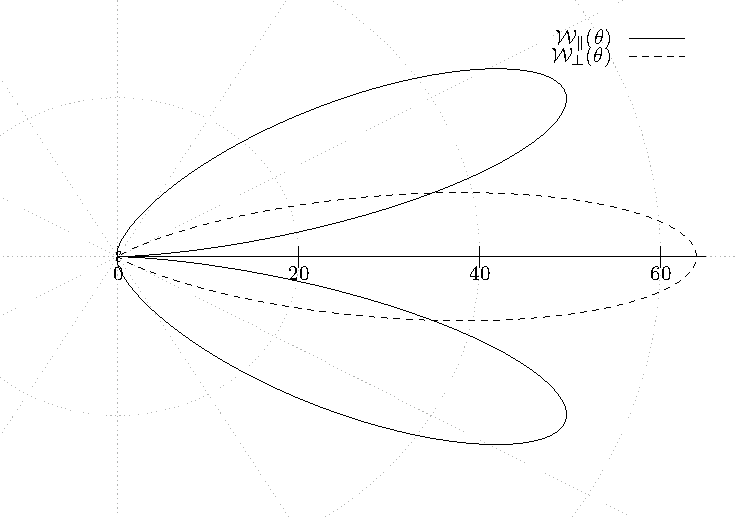
\includegraphics[width=\linewidth]{perp_par.pdf}
% \documentclass[10pt]{article}
\usepackage[T1]{fontenc}
\usepackage{textcomp}

\usepackage[utf8x]{inputenc}
\SetUnicodeOption{mathletters}

\usepackage{gnuplot-lua-tikz}
\pagestyle{empty}
\usepackage[active,tightpage]{preview}
\PreviewEnvironment{tikzpicture}
\setlength\PreviewBorder{\gpbboxborder}
\begin{document}

\begin{tikzpicture}[gnuplot]
%% generated with GNUPLOT 5.2p0 (Lua 5.3; terminal rev. 99, script rev. 102)
%% Вт 09 янв 2018 19:23:20
\gpmonochromelines
\path (0.000,0.000) rectangle (12.500,8.750);
\gpcolor{color=gp lt color border}
\gpsetlinetype{gp lt border}
\gpsetdashtype{gp dt solid}
\gpsetlinewidth{1.00}
\draw[gp path] (1.992,4.405)--(1.992,4.585);
\draw[gp path] (1.992,4.405)--(1.992,4.225);
\node[gp node center] at (1.992,4.097) {$0$};
\gpcolor{color=gp lt color axes}
\gpsetlinetype{gp lt axes}
\gpsetdashtype{gp dt axes}
\gpsetlinewidth{0.50}
\draw[gp path] (5.055,4.405)--(5.052,4.522)--(5.043,4.639)--(5.029,4.756)--(5.008,4.872)%
  --(4.982,4.987)--(4.950,5.101)--(4.913,5.214)--(4.870,5.325)--(4.822,5.434)--(4.768,5.542)%
  --(4.709,5.647)--(4.644,5.750)--(4.575,5.850)--(4.501,5.948)--(4.422,6.043)--(4.338,6.134)%
  --(4.250,6.223)--(4.158,6.307)--(4.061,6.389)--(3.961,6.466)--(3.856,6.539)--(3.749,6.609)%
  --(3.637,6.674)--(3.523,6.735)--(3.406,6.791)--(3.286,6.843)--(3.164,6.891)--(3.039,6.933)%
  --(2.913,6.971)--(2.784,7.004)--(2.655,7.032)--(2.524,7.055)--(2.391,7.072)--(2.259,7.085)%
  --(2.125,7.093)--(1.992,7.096)--(1.858,7.093)--(1.725,7.085)--(1.592,7.072)--(1.460,7.055)%
  --(1.329,7.032)--(1.199,7.004)--(1.070,6.971)--(0.944,6.933)--(0.819,6.891)--(0.697,6.843)%
  --(0.577,6.791)--(0.460,6.735)--(0.346,6.674)--(0.235,6.609)--(0.127,6.539)--(0.023,6.466)%
  --(0.000,6.448);
\draw[gp path] (0.000,2.360)--(0.023,2.343)--(0.127,2.270)--(0.235,2.200)--(0.346,2.135)%
  --(0.460,2.074)--(0.577,2.018)--(0.697,1.966)--(0.819,1.918)--(0.944,1.876)--(1.070,1.838)%
  --(1.199,1.805)--(1.329,1.777)--(1.460,1.754)--(1.592,1.737)--(1.725,1.724)--(1.858,1.716)%
  --(1.992,1.714)--(2.125,1.716)--(2.259,1.724)--(2.391,1.737)--(2.524,1.754)--(2.655,1.777)%
  --(2.784,1.805)--(2.913,1.838)--(3.039,1.876)--(3.164,1.918)--(3.286,1.966)--(3.406,2.018)%
  --(3.523,2.074)--(3.637,2.135)--(3.749,2.200)--(3.856,2.270)--(3.961,2.343)--(4.061,2.420)%
  --(4.158,2.502)--(4.250,2.586)--(4.338,2.675)--(4.422,2.766)--(4.501,2.861)--(4.575,2.959)%
  --(4.644,3.059)--(4.709,3.162)--(4.768,3.267)--(4.822,3.375)--(4.870,3.484)--(4.913,3.595)%
  --(4.950,3.708)--(4.982,3.822)--(5.008,3.937)--(5.029,4.053)--(5.043,4.170)--(5.052,4.287)%
  --(5.055,4.404);
\gpcolor{color=gp lt color border}
\gpsetlinetype{gp lt border}
\gpsetdashtype{gp dt solid}
\gpsetlinewidth{1.00}
\draw[gp path] (5.055,4.405)--(5.055,4.585);
\draw[gp path] (5.055,4.405)--(5.055,4.225);
\node[gp node center] at (5.055,4.097) {$20$};
\gpcolor{color=gp lt color axes}
\gpsetlinetype{gp lt axes}
\gpsetdashtype{gp dt axes}
\gpsetlinewidth{0.50}
\draw[gp path] (8.118,4.405)--(8.112,4.639)--(8.095,4.874)--(8.066,5.107)--(8.025,5.339)%
  --(7.973,5.569)--(7.909,5.797)--(7.834,6.023)--(7.749,6.245)--(7.652,6.464)--(7.544,6.679)%
  --(7.426,6.890)--(7.297,7.096)--(7.159,7.296)--(7.010,7.491)--(6.852,7.681)--(6.685,7.864)%
  --(6.508,8.041)--(6.324,8.210)--(6.131,8.373)--(5.930,8.527)--(5.721,8.674)--(5.604,8.749);
\draw[gp path] (5.510,0.000)--(5.721,0.135)--(5.930,0.282)--(6.131,0.436)--(6.324,0.599)%
  --(6.508,0.768)--(6.685,0.945)--(6.852,1.128)--(7.010,1.318)--(7.159,1.513)--(7.297,1.713)%
  --(7.426,1.919)--(7.544,2.130)--(7.652,2.345)--(7.749,2.564)--(7.834,2.786)--(7.909,3.012)%
  --(7.973,3.240)--(8.025,3.470)--(8.066,3.702)--(8.095,3.935)--(8.112,4.170)--(8.118,4.404);
\gpcolor{color=gp lt color border}
\gpsetlinetype{gp lt border}
\gpsetdashtype{gp dt solid}
\gpsetlinewidth{1.00}
\draw[gp path] (8.118,4.405)--(8.118,4.585);
\draw[gp path] (8.118,4.405)--(8.118,4.225);
\node[gp node center] at (8.118,4.097) {$40$};
\gpcolor{color=gp lt color axes}
\gpsetlinetype{gp lt axes}
\gpsetdashtype{gp dt axes}
\gpsetlinewidth{0.50}
\draw[gp path] (11.181,4.405)--(11.172,4.757)--(11.146,5.108)--(11.103,5.458)--(11.042,5.806)%
  --(10.963,6.152)--(10.868,6.494)--(10.756,6.832)--(10.627,7.166)--(10.482,7.494)--(10.320,7.816)%
  --(10.143,8.132)--(9.950,8.441)--(9.742,8.742)--(9.736,8.749);
\draw[gp path] (9.690,0.000)--(9.742,0.067)--(9.950,0.368)--(10.143,0.677)--(10.320,0.993)%
  --(10.482,1.315)--(10.627,1.643)--(10.756,1.977)--(10.868,2.315)--(10.963,2.657)--(11.042,3.003)%
  --(11.103,3.351)--(11.146,3.701)--(11.172,4.052)--(11.181,4.404);
\gpcolor{color=gp lt color border}
\gpsetlinetype{gp lt border}
\gpsetdashtype{gp dt solid}
\gpsetlinewidth{1.00}
\draw[gp path] (11.181,4.405)--(11.181,4.585);
\draw[gp path] (11.181,4.405)--(11.181,4.225);
\node[gp node center] at (11.181,4.097) {$60$};
\gpcolor{color=gp lt color axes}
\gpsetlinetype{gp lt axes}
\gpsetdashtype{gp dt axes}
\gpsetlinewidth{0.50}
\draw[gp path] (1.992,4.405)--(12.499,4.405);
\draw[gp path] (1.992,4.405)--(10.558,8.749);
\draw[gp path] (1.992,4.405)--(4.846,8.749);
\draw[gp path] (1.992,4.405)--(1.992,8.749);
\draw[gp path] (1.992,4.405)--(0.000,7.435);
\draw[gp path] (1.992,4.405)--(0.000,5.415);
\draw[gp path] (1.992,4.405)--(0.000,4.405);
\draw[gp path] (1.992,4.405)--(0.000,3.394);
\draw[gp path] (1.992,4.405)--(0.000,1.374);
\draw[gp path] (1.992,4.405)--(1.992,0.000);
\draw[gp path] (1.992,4.405)--(4.887,0.000);
\draw[gp path] (1.992,4.405)--(10.678,0.000);
\draw[gp path] (1.992,4.405)--(12.499,4.405);
\gpcolor{color=gp lt color border}
\node[gp node right] at (10.479,8.107) {$\mathcal W_\parallel(\theta)$};
\gpsetlinetype{gp lt border}
\gpsetdashtype{gp dt solid}
\gpsetlinewidth{1.00}
\draw[gp path] (10.663,8.107)--(11.579,8.107);
\draw[gp path] (1.992,4.405)--(2.016,4.405)--(2.091,4.407)--(2.213,4.412)--(2.381,4.422)%
  --(2.593,4.438)--(2.845,4.461)--(3.134,4.493)--(3.455,4.534)--(3.803,4.586)--(4.174,4.647)%
  --(4.562,4.719)--(4.961,4.802)--(5.367,4.894)--(5.775,4.997)--(6.179,5.108)--(6.575,5.227)%
  --(6.958,5.353)--(7.324,5.485)--(7.670,5.621)--(7.992,5.761)--(8.289,5.902)--(8.557,6.044)%
  --(8.796,6.186)--(9.004,6.325)--(9.180,6.461)--(9.324,6.592)--(9.436,6.718)--(9.517,6.837)%
  --(9.568,6.949)--(9.590,7.053)--(9.583,7.149)--(9.551,7.235)--(9.493,7.312)--(9.413,7.380)%
  --(9.312,7.438)--(9.192,7.486)--(9.055,7.524)--(8.902,7.553)--(8.737,7.573)--(8.560,7.584)%
  --(8.374,7.587)--(8.180,7.582)--(7.980,7.568)--(7.776,7.548)--(7.568,7.521)--(7.359,7.488)%
  --(7.148,7.450)--(6.939,7.406)--(6.730,7.357)--(6.524,7.305)--(6.321,7.249)--(6.121,7.190)%
  --(5.926,7.128)--(5.735,7.063)--(5.549,6.997)--(5.369,6.930)--(5.195,6.861)--(5.026,6.792)%
  --(4.864,6.722)--(4.708,6.652)--(4.557,6.582)--(4.413,6.512)--(4.276,6.443)--(4.144,6.374)%
  --(4.018,6.306)--(3.898,6.240)--(3.784,6.174)--(3.676,6.110)--(3.572,6.047)--(3.475,5.985)%
  --(3.382,5.925)--(3.294,5.866)--(3.211,5.809)--(3.133,5.754)--(3.059,5.700)--(2.989,5.648)%
  --(2.923,5.597)--(2.861,5.548)--(2.802,5.501)--(2.747,5.455)--(2.695,5.411)--(2.647,5.369)%
  --(2.601,5.328)--(2.558,5.288)--(2.518,5.250)--(2.480,5.214)--(2.445,5.178)--(2.412,5.145)%
  --(2.381,5.112)--(2.352,5.081)--(2.325,5.051)--(2.299,5.023)--(2.276,4.995)--(2.254,4.969)%
  --(2.233,4.944)--(2.214,4.920)--(2.196,4.897)--(2.179,4.874)--(2.163,4.853)--(2.149,4.833)%
  --(2.135,4.814)--(2.123,4.795)--(2.111,4.777)--(2.100,4.761)--(2.090,4.744)--(2.080,4.729)%
  --(2.072,4.714)--(2.064,4.700)--(2.056,4.687)--(2.049,4.674)--(2.043,4.661)--(2.037,4.650)%
  --(2.031,4.638)--(2.026,4.628)--(2.022,4.617)--(2.017,4.608)--(2.013,4.598)--(2.010,4.589)%
  --(2.006,4.581)--(2.003,4.573)--(2.000,4.565)--(1.998,4.558)--(1.995,4.551)--(1.993,4.544)%
  --(1.991,4.537)--(1.989,4.531)--(1.988,4.525)--(1.986,4.520)--(1.985,4.515)--(1.984,4.509)%
  --(1.983,4.505)--(1.982,4.500)--(1.981,4.496)--(1.980,4.491)--(1.979,4.487)--(1.979,4.483)%
  --(1.978,4.480)--(1.978,4.476)--(1.977,4.473)--(1.977,4.470)--(1.977,4.467)--(1.977,4.464)%
  --(1.977,4.461)--(1.976,4.458)--(1.976,4.456)--(1.976,4.453)--(1.976,4.451)--(1.976,4.449)%
  --(1.976,4.447)--(1.977,4.445)--(1.977,4.443)--(1.977,4.441)--(1.977,4.439)--(1.977,4.438)%
  --(1.977,4.436)--(1.977,4.434)--(1.978,4.433)--(1.978,4.432)--(1.978,4.430)--(1.978,4.429)%
  --(1.979,4.428)--(1.979,4.427)--(1.979,4.426)--(1.979,4.425)--(1.980,4.424)--(1.980,4.423)%
  --(1.980,4.422)--(1.980,4.421)--(1.981,4.420)--(1.981,4.419)--(1.981,4.418)--(1.982,4.417)%
  --(1.982,4.416)--(1.982,4.415)--(1.983,4.415)--(1.983,4.414)--(1.983,4.413)--(1.984,4.413)%
  --(1.984,4.412)--(1.984,4.411)--(1.985,4.411)--(1.985,4.410)--(1.986,4.410)--(1.986,4.409)%
  --(1.986,4.408)--(1.987,4.408)--(1.987,4.407)--(1.988,4.407)--(1.988,4.406)--(1.989,4.406)%
  --(1.989,4.405)--(1.990,4.405)--(1.991,4.405)--(1.992,4.405)--(1.992,4.404)--(1.991,4.404)%
  --(1.990,4.404)--(1.989,4.404)--(1.989,4.403)--(1.988,4.403)--(1.988,4.402)--(1.987,4.402)%
  --(1.987,4.401)--(1.986,4.401)--(1.986,4.400)--(1.986,4.399)--(1.985,4.399)--(1.985,4.398)%
  --(1.984,4.398)--(1.984,4.397)--(1.984,4.396)--(1.983,4.396)--(1.983,4.395)--(1.983,4.394)%
  --(1.982,4.394)--(1.982,4.393)--(1.982,4.392)--(1.981,4.391)--(1.981,4.390)--(1.981,4.389)%
  --(1.980,4.388)--(1.980,4.387)--(1.980,4.386)--(1.980,4.385)--(1.979,4.384)--(1.979,4.383)%
  --(1.979,4.382)--(1.979,4.381)--(1.978,4.380)--(1.978,4.379)--(1.978,4.377)--(1.978,4.376)%
  --(1.977,4.375)--(1.977,4.373)--(1.977,4.371)--(1.977,4.370)--(1.977,4.368)--(1.977,4.366)%
  --(1.977,4.364)--(1.976,4.362)--(1.976,4.360)--(1.976,4.358)--(1.976,4.356)--(1.976,4.353)%
  --(1.976,4.351)--(1.977,4.348)--(1.977,4.345)--(1.977,4.342)--(1.977,4.339)--(1.977,4.336)%
  --(1.978,4.333)--(1.978,4.329)--(1.979,4.326)--(1.979,4.322)--(1.980,4.318)--(1.981,4.313)%
  --(1.982,4.309)--(1.983,4.304)--(1.984,4.300)--(1.985,4.294)--(1.986,4.289)--(1.988,4.284)%
  --(1.989,4.278)--(1.991,4.272)--(1.993,4.265)--(1.995,4.258)--(1.998,4.251)--(2.000,4.244)%
  --(2.003,4.236)--(2.006,4.228)--(2.010,4.220)--(2.013,4.211)--(2.017,4.201)--(2.022,4.192)%
  --(2.026,4.181)--(2.031,4.171)--(2.037,4.159)--(2.043,4.148)--(2.049,4.135)--(2.056,4.122)%
  --(2.064,4.109)--(2.072,4.095)--(2.080,4.080)--(2.090,4.065)--(2.100,4.048)--(2.111,4.032)%
  --(2.123,4.014)--(2.135,3.995)--(2.149,3.976)--(2.163,3.956)--(2.179,3.935)--(2.196,3.912)%
  --(2.214,3.889)--(2.233,3.865)--(2.254,3.840)--(2.276,3.814)--(2.299,3.786)--(2.325,3.758)%
  --(2.352,3.728)--(2.381,3.697)--(2.412,3.664)--(2.445,3.631)--(2.480,3.595)--(2.518,3.559)%
  --(2.558,3.521)--(2.601,3.481)--(2.647,3.440)--(2.695,3.398)--(2.747,3.354)--(2.802,3.308)%
  --(2.861,3.261)--(2.923,3.212)--(2.989,3.161)--(3.059,3.109)--(3.133,3.055)--(3.211,3.000)%
  --(3.294,2.943)--(3.382,2.884)--(3.475,2.824)--(3.572,2.762)--(3.676,2.699)--(3.784,2.635)%
  --(3.898,2.569)--(4.018,2.503)--(4.144,2.435)--(4.276,2.366)--(4.413,2.297)--(4.557,2.227)%
  --(4.708,2.157)--(4.864,2.087)--(5.026,2.017)--(5.195,1.948)--(5.369,1.879)--(5.549,1.812)%
  --(5.735,1.746)--(5.926,1.681)--(6.121,1.619)--(6.321,1.560)--(6.524,1.504)--(6.730,1.452)%
  --(6.939,1.403)--(7.148,1.359)--(7.359,1.321)--(7.568,1.288)--(7.776,1.261)--(7.980,1.241)%
  --(8.180,1.227)--(8.374,1.222)--(8.560,1.225)--(8.737,1.236)--(8.902,1.256)--(9.055,1.285)%
  --(9.192,1.323)--(9.312,1.371)--(9.413,1.429)--(9.493,1.497)--(9.551,1.574)--(9.583,1.660)%
  --(9.590,1.756)--(9.568,1.860)--(9.517,1.972)--(9.436,2.091)--(9.324,2.217)--(9.180,2.348)%
  --(9.004,2.484)--(8.796,2.623)--(8.557,2.765)--(8.289,2.907)--(7.992,3.048)--(7.670,3.188)%
  --(7.324,3.324)--(6.958,3.456)--(6.575,3.582)--(6.179,3.701)--(5.775,3.812)--(5.367,3.915)%
  --(4.961,4.007)--(4.562,4.090)--(4.174,4.162)--(3.803,4.223)--(3.455,4.275)--(3.134,4.316)%
  --(2.845,4.348)--(2.593,4.371)--(2.381,4.387)--(2.213,4.397)--(2.091,4.402)--(2.016,4.404)%
  --cycle;
\node[gp node right] at (10.479,7.799) {$\mathcal W_\perp(\theta)$};
\gpsetdashtype{gp dt 2}
\draw[gp path] (10.663,7.799)--(11.579,7.799);
\draw[gp path] (11.794,4.405)--(11.775,4.513)--(11.720,4.620)--(11.627,4.724)--(11.500,4.826)%
  --(11.339,4.922)--(11.146,5.013)--(10.923,5.098)--(10.672,5.175)--(10.397,5.245)--(10.100,5.306)%
  --(9.785,5.359)--(9.454,5.403)--(9.110,5.437)--(8.757,5.463)--(8.397,5.480)--(8.035,5.489)%
  --(7.671,5.489)--(7.310,5.482)--(6.954,5.468)--(6.604,5.447)--(6.263,5.421)--(5.932,5.389)%
  --(5.614,5.353)--(5.308,5.313)--(5.017,5.270)--(4.740,5.225)--(4.479,5.178)--(4.234,5.129)%
  --(4.005,5.081)--(3.791,5.032)--(3.593,4.983)--(3.411,4.936)--(3.244,4.890)--(3.090,4.845)%
  --(2.951,4.802)--(2.825,4.761)--(2.712,4.723)--(2.610,4.686)--(2.519,4.652)--(2.438,4.621)%
  --(2.367,4.592)--(2.304,4.565)--(2.250,4.541)--(2.202,4.519)--(2.162,4.500)--(2.127,4.482)%
  --(2.097,4.467)--(2.073,4.454)--(2.053,4.442)--(2.036,4.433)--(2.023,4.425)--(2.012,4.419)%
  --(2.005,4.413)--(1.999,4.410)--(1.995,4.407)--(1.993,4.405)--(1.992,4.405)--(1.993,4.405)%
  --(1.994,4.407)--(1.997,4.409)--(1.999,4.411)--(2.002,4.414)--(2.005,4.417)--(2.008,4.420)%
  --(2.012,4.424)--(2.015,4.428)--(2.018,4.431)--(2.021,4.435)--(2.024,4.439)--(2.027,4.443)%
  --(2.029,4.447)--(2.031,4.450)--(2.033,4.454)--(2.035,4.457)--(2.037,4.461)--(2.038,4.464)%
  --(2.039,4.467)--(2.040,4.470)--(2.041,4.473)--(2.041,4.476)--(2.042,4.478)--(2.042,4.480)%
  --(2.042,4.483)--(2.042,4.485)--(2.041,4.487)--(2.041,4.488)--(2.040,4.490)--(2.039,4.491)%
  --(2.038,4.492)--(2.037,4.493)--(2.036,4.494)--(2.035,4.495)--(2.034,4.496)--(2.033,4.496)%
  --(2.031,4.497)--(2.030,4.497)--(2.029,4.497)--(2.027,4.497)--(2.026,4.497)--(2.024,4.497)%
  --(2.023,4.497)--(2.021,4.497)--(2.020,4.497)--(2.018,4.496)--(2.017,4.496)--(2.015,4.495)%
  --(2.014,4.495)--(2.012,4.494)--(2.011,4.494)--(2.009,4.493)--(2.008,4.492)--(2.006,4.491)%
  --(2.005,4.490)--(2.004,4.490)--(2.002,4.489)--(2.001,4.488)--(2.000,4.487)--(1.998,4.486)%
  --(1.997,4.485)--(1.996,4.484)--(1.995,4.483)--(1.994,4.482)--(1.992,4.481)--(1.991,4.480)%
  --(1.990,4.479)--(1.989,4.478)--(1.988,4.477)--(1.987,4.476)--(1.986,4.475)--(1.985,4.474)%
  --(1.985,4.473)--(1.984,4.472)--(1.983,4.471)--(1.982,4.469)--(1.981,4.468)--(1.980,4.467)%
  --(1.980,4.466)--(1.979,4.465)--(1.978,4.464)--(1.978,4.463)--(1.977,4.462)--(1.976,4.461)%
  --(1.976,4.460)--(1.975,4.459)--(1.974,4.458)--(1.974,4.457)--(1.973,4.456)--(1.973,4.455)%
  --(1.972,4.454)--(1.972,4.453)--(1.971,4.452)--(1.971,4.451)--(1.971,4.450)--(1.970,4.450)%
  --(1.970,4.449)--(1.970,4.448)--(1.969,4.447)--(1.969,4.446)--(1.968,4.445)--(1.968,4.444)%
  --(1.968,4.443)--(1.967,4.442)--(1.967,4.441)--(1.967,4.440)--(1.966,4.439)--(1.966,4.438)%
  --(1.966,4.437)--(1.966,4.436)--(1.965,4.435)--(1.965,4.434)--(1.965,4.433)--(1.965,4.432)%
  --(1.965,4.431)--(1.964,4.430)--(1.964,4.429)--(1.964,4.428)--(1.964,4.427)--(1.964,4.426)%
  --(1.964,4.425)--(1.964,4.424)--(1.964,4.423)--(1.963,4.422)--(1.963,4.421)--(1.963,4.420)%
  --(1.963,4.419)--(1.963,4.418)--(1.963,4.417)--(1.963,4.416)--(1.963,4.415)--(1.963,4.414)%
  --(1.963,4.413)--(1.963,4.412)--(1.963,4.411)--(1.963,4.410)--(1.963,4.409)--(1.963,4.408)%
  --(1.963,4.407)--(1.963,4.406)--(1.963,4.405)--(1.963,4.404)--(1.963,4.403)--(1.963,4.402)%
  --(1.963,4.401)--(1.963,4.400)--(1.963,4.399)--(1.963,4.398)--(1.963,4.397)--(1.963,4.396)%
  --(1.963,4.395)--(1.963,4.394)--(1.963,4.393)--(1.963,4.392)--(1.963,4.391)--(1.963,4.390)%
  --(1.963,4.389)--(1.963,4.388)--(1.963,4.387)--(1.964,4.386)--(1.964,4.385)--(1.964,4.384)%
  --(1.964,4.383)--(1.964,4.382)--(1.964,4.381)--(1.964,4.380)--(1.964,4.379)--(1.965,4.378)%
  --(1.965,4.377)--(1.965,4.376)--(1.965,4.375)--(1.965,4.374)--(1.966,4.373)--(1.966,4.372)%
  --(1.966,4.371)--(1.966,4.370)--(1.967,4.369)--(1.967,4.368)--(1.967,4.367)--(1.968,4.366)%
  --(1.968,4.365)--(1.968,4.364)--(1.969,4.363)--(1.969,4.362)--(1.970,4.361)--(1.970,4.360)%
  --(1.970,4.359)--(1.971,4.359)--(1.971,4.358)--(1.971,4.357)--(1.972,4.356)--(1.972,4.355)%
  --(1.973,4.354)--(1.973,4.353)--(1.974,4.352)--(1.974,4.351)--(1.975,4.350)--(1.976,4.349)%
  --(1.976,4.348)--(1.977,4.347)--(1.978,4.346)--(1.978,4.345)--(1.979,4.344)--(1.980,4.343)%
  --(1.980,4.342)--(1.981,4.341)--(1.982,4.340)--(1.983,4.338)--(1.984,4.337)--(1.985,4.336)%
  --(1.985,4.335)--(1.986,4.334)--(1.987,4.333)--(1.988,4.332)--(1.989,4.331)--(1.990,4.330)%
  --(1.991,4.329)--(1.992,4.328)--(1.994,4.327)--(1.995,4.326)--(1.996,4.325)--(1.997,4.324)%
  --(1.998,4.323)--(2.000,4.322)--(2.001,4.321)--(2.002,4.320)--(2.004,4.319)--(2.005,4.319)%
  --(2.006,4.318)--(2.008,4.317)--(2.009,4.316)--(2.011,4.315)--(2.012,4.315)--(2.014,4.314)%
  --(2.015,4.314)--(2.017,4.313)--(2.018,4.313)--(2.020,4.312)--(2.021,4.312)--(2.023,4.312)%
  --(2.024,4.312)--(2.026,4.312)--(2.027,4.312)--(2.029,4.312)--(2.030,4.312)--(2.031,4.312)%
  --(2.033,4.313)--(2.034,4.313)--(2.035,4.314)--(2.036,4.315)--(2.037,4.316)--(2.038,4.317)%
  --(2.039,4.318)--(2.040,4.319)--(2.041,4.321)--(2.041,4.322)--(2.042,4.324)--(2.042,4.326)%
  --(2.042,4.329)--(2.042,4.331)--(2.041,4.333)--(2.041,4.336)--(2.040,4.339)--(2.039,4.342)%
  --(2.038,4.345)--(2.037,4.348)--(2.035,4.352)--(2.033,4.355)--(2.031,4.359)--(2.029,4.362)%
  --(2.027,4.366)--(2.024,4.370)--(2.021,4.374)--(2.018,4.378)--(2.015,4.381)--(2.012,4.385)%
  --(2.008,4.389)--(2.005,4.392)--(2.002,4.395)--(1.999,4.398)--(1.997,4.400)--(1.994,4.402)%
  --(1.993,4.404)--(1.992,4.404)--(1.993,4.404)--(1.995,4.402)--(1.999,4.399)--(2.005,4.396)%
  --(2.012,4.390)--(2.023,4.384)--(2.036,4.376)--(2.053,4.367)--(2.073,4.355)--(2.097,4.342)%
  --(2.127,4.327)--(2.162,4.309)--(2.202,4.290)--(2.250,4.268)--(2.304,4.244)--(2.367,4.217)%
  --(2.438,4.188)--(2.519,4.157)--(2.610,4.123)--(2.712,4.086)--(2.825,4.048)--(2.951,4.007)%
  --(3.090,3.964)--(3.244,3.919)--(3.411,3.873)--(3.593,3.826)--(3.791,3.777)--(4.005,3.728)%
  --(4.234,3.680)--(4.479,3.631)--(4.740,3.584)--(5.017,3.539)--(5.308,3.496)--(5.614,3.456)%
  --(5.932,3.420)--(6.263,3.388)--(6.604,3.362)--(6.954,3.341)--(7.310,3.327)--(7.671,3.320)%
  --(8.035,3.320)--(8.397,3.329)--(8.757,3.346)--(9.110,3.372)--(9.454,3.406)--(9.785,3.450)%
  --(10.100,3.503)--(10.397,3.564)--(10.672,3.634)--(10.923,3.711)--(11.146,3.796)--(11.339,3.887)%
  --(11.500,3.983)--(11.627,4.085)--(11.720,4.189)--(11.775,4.296)--(11.794,4.404);
\gpsetdashtype{gp dt solid}
\draw[gp path] (1.992,4.405)--(11.947,4.405);
%% coordinates of the plot area
\gpdefrectangularnode{gp plot 1}{\pgfpoint{0.460cm}{0.368cm}}{\pgfpoint{11.947cm}{8.441cm}}
\end{tikzpicture}
%% gnuplot variables
\end{document}


\begin{enumerate}
  \item $\mathcal W_\parallel = \frac{e^2}{4\pi c^2} \, w^2 \, \frac{\sin^2\theta}{(1-\beta \cos \theta)^5}$, $\theta_0 \approx \frac{1}{2 \gamma}$
  \item $\mathcal W_\perp = \frac{e^2}{4\pi c^2}  \, \frac{w^2}{{(1-\beta \cos \theta)}^3} 
  \left(1 - \frac{\sin^2 \theta \, \cos^2 \varphi}{\gamma^2\, {(1-\beta \, \cos \theta)}^2}\right)$,
    $\theta_0 = 0$, $\Delta \theta \approx 1/\gamma$
\end{enumerate}

$\gamma \gg 1 \quad I \approx I_\perp$

$\Delta t_1 \sim \frac{\rho}{c \gamma} \Rightarrow \Delta t \sim \frac{\rho}{c \gamma^3}  
\Rightarrow \omega < \omega_c = \frac{c \gamma^3}{\rho}$ 

\paragraph{Спектр и поляризация движения по окружности}
\underdev \flame

\begin{enumerate}
  \item $\v M := \sqrt{c \over 4\pi}$, $\mathcal W(\v n, t) = |\v S|\, R^2 = |\v M(t)|^2 =
    \fder{\mathcal E(t)}{t}$
  \item $\v M(\omega) = \frac{e}{c} \, \sqrt{c \over 4\pi} \intR e^{i \omega t} \,\del
    \left(\frac{\v n \times (\v n \times \v \beta)}{1 - \v n \cdot \v \beta}\right)$
  \item $t = T + R/c = t_1 - \frac 1c \v n\cdot \v x$
  \item $\v M(\omega) = \frac{-i\omega e\, e^{i \omega R}}{c} \, \sqrt{c \over 4\pi} \* 
     \intR e^{i \omega (t_1 - \frac 1c \v n \cdot \v \beta)} \,
  \v n \times (\v n \times \v \beta)\, \del t_1$
  \item В поляризационном базисе и при малых углах
    \begin{small}
      $
      \begin{aligned}
        \varepsilon (\omega, \theta) &= \frac{e^2 \omega^2}{4\pi^2 c}\,|-\v e_\parallel M_\parallel + \v e_\perp M_\perp|\\
        \varepsilon (\omega, \theta) &= \frac{e^2}{3\pi^2 c} \*
        {\left(\frac{\omega \rho}{x}\right)}^2 \* {\left(\frac 1{\gamma^2} + \theta^2 \right)}^2\*
        \left\lvert \mathcal K_{2/3}^2 (\xi) + \tfrac{u^2}{1+u^2}\, \mathcal K_{1/3}^2 (\xi)\right\rvert\\
        u &= \gamma \theta, \quad
        x = \frac{ct}{\rho} \, {\left(\tfrac{1}{\gamma^2} + \theta^2\right)}^{-1/2} \;
        \xi = \frac{\omega \rho}{3c}\, {\left(\tfrac{1}{\gamma^2} + \theta^2\right)}^{3/2} \\
        & w_c = 3 \gamma^3 \omega_0,\quad \omega_0 = \rho/c
      \end{aligned}
      $
    \end{small}
\end{enumerate}

$\int \varepsilon(\omega, \theta) \, \del \omega = \frac{7}{16} \, \frac{e^2}{\rho} \, 
\frac{\gamma^5}{{\bigl(1 + (\gamma \theta)\bigr)}^{5/2}} \, \left( 1 + \frac{5 u^2}{7\,(1+u^2)}\right)$

$\int \del \Omega \, \int \varepsilon (\omega,\theta) \, \del \omega 
= \frac{7 \pi e^2 \gamma^4}{4 \rho} \left(I_2 + \frac 57\bigl(I_2 - I_3\bigr)\right)$

\plholdev{возня с асимптотикой \underdev}
\paragraph{Магнитотормозное излучение}
\underdev\ \flame%

$\v E = 0 \Rightarrow \fder{\mathcal E}{t} = e \v v \cdot \v E = 0$

\begin{defs}[Ларморовская частота]
\item[Ларморовская частота] $\omega_H = \frac{e H}{mc \gamma}$ 
\item[Циклотронная частота] $\frac{e H}{mc}$ 
\item[Ларморовский радиус] $\rho_H = \frac{v_\perp}{\omega_H} = \frac{v \, \sin \chi}{\omega_H}$
\end{defs}

\begin{facts}
\item $w = \omega_H v\, \sin \chi $
\item $\left\{
  \begin{aligned}
    x &= x_0 + \rho_H \, \sin(\omega_H t + \alpha) \\
    y &= y_0 + \rho_H \, \cos(\omega_H t + \alpha)\\
    z &= z_0 + v\, \cos \chi \, t
\end{aligned}\right.
  $~--- спиралька 
\item $F_\parallel= 0 \Rightarrow I = \frac{2 e^4 v^2 H^2 \sin^2 \chi}{3m^2 c^5} \propto \frac{e^4}{m^2}$
\item $\mathcal W_{\text{набл}} = \frac{1}{\sin^2 \chi} \,\mathcal W_{\text{исп}}$
\end{facts}

А что такое $W$ я не знаю. И не знаю, узнаю ли. Приятного использования.
\begin{small}
  \begin{enumerate}
    \item $\v M (t) \sum^{\infty}_{k=-\infty} \v M_k e^{-i \omega_H k t} $
    \item $W_k(\theta) = \frac{e^2k^2 \omega_H^2}{2\pi c}\,
      \Bigl\lvert\v e_\parallel \beta J_k'(k \beta \cos \theta) + i \v e_\perp \tg \theta \, J_k (k \beta \cos \theta)\Bigr\rvert^2$
      (формула Шотта)
    \item при $\theta = 0$ переходит в линейную, при $\theta = \pi/2$~"--- в круговую.\note{Угол между направлением и плоскостью 
      движения, так-то.}
  \end{enumerate}
\end{small}

\plholdev{дурацкие частные случаи}

\paragraph{Рассеяние на свободных зарядах}
\begin{defs}[комптоновская длина]
\item[классический радиус электрона] $r_e= \frac{e^2}{mc^2}$
\item[комптоновская длина волны] $\lambda_c = \frac{h}{mc}$
 \end{defs}

\begin{facts}
\item $\v E = {(E_1, E_2)}^\top$, $r_e= \frac{e^2}{mc^2}$~--- классический радиус электрона
\item $A = \begin{pmatrix} \mu & 0 \\ 0 & 1 \end{pmatrix}$, $\v E = \frac{r_e}{R}  A \, \v E'$, $\rho = \frac{r_e^2}{R^2} \, A \rho' A$
  \item $\v I = \frac{r_e^2}{R^2} \, R(\mu) \v I'$, а $R = \begin{pmatrix}
    \frac{\mu^2 + 1}{2}  &  \frac{{\mu^2 - 1}}{2}  & 0 & 0 \\
      \frac{\mu^2 - 1}{2}  &  \frac{{\mu^2 + 1}}{2} & 0 & 0 \\
      0 & 0 & \mu & 0 \\
      0 & 0 & 0 & \mu
  \end{pmatrix}$
\item Для белого света ($I'$) $I = \frac{r_e^2}{2R^2}\, (1 + \mu^2) I'$
\end{facts}

\begin{defs}[дифференциальное]
\item[дифференциальное сечение рассеяния] $\del \sigma = I \, \del \Omega $
\item[сечение рассеяния] $\sigma_0 = \int \del \sigma $
\end{defs}

\begin{itemize}
  \item В классике: $\del \sigma = \frac{r_e^2}{2}\, (1+\mu^2) \, \del \Omega $
  \item $\sigma_0 = \frac 83 \pi r_e^2$
  \item В квантах: $\del \sigma = \frac{r_e^2}{2}  {\left(\frac{\omega'}{\omega}\right)}^2
    \left(\frac{\omega'}{\Omega} +\frac{\omega'}{\Omega} - \sin^2 \theta \right) \, \del \Omega $
\end{itemize}

\paragraph{Влияние излучение на движение}

$m (\dot{\v v} - \tau \ddot{\v v})= \v F_{\mathrm{ex}}$~--- уравнение Абрагама-Лоренца.

Имеет смысл при $\bigl\lvert \v F_{\mathrm{rad}} \bigr\rvert \ll \bigl\lvert \v F_{\mathrm{ex}} \bigr\rvert$. 
А всё остальное в этом билете не имеет смысла.

\paragraph{Радиационное затухание}
\begin{facts}
\item $m \tau \omega_0^2 \, \dddot{x} = - \gamma m \dot x$, $\gamma = \tau \omega_0^2 \,\frac{2}{3}\, \frac{e^2}{c^3m}$
\item $\v x = \v a \, e^{-i \omega t}\, e^{-\gamma t/2}$, $1/\gamma$~"--- характерное время убывания. 
\item $I = \frac{\lfrac{\gamma\, I_0}{2\pi}}{{(\omega - \omega_0)}^2 + \lfrac{\gamma^2} 4}$~--- лоренцевский контур линии
\end{facts}
\noindent
\begin{tikzpicture}
    \def\wz{1}\def\g{0.2}
  \begin{axis}[
   xlabel=$\omega$, ylabel=$\tfrac{I}{I_{\textrm{max}}}$, 
    domain = (\wz - 4*\g):(\wz + 4*\g),
    ymin = 0, ymax = 100,
    width=0.9\linewidth,
    height=0.6\linewidth,
    axis y line=left,
    axis x line=bottom, 
    grid=both,
    grid style={line width=.1pt, draw=gray!10},
    major grid style={line width=.2pt,draw=gray!40},
    minor tick num=1,
    ]
    % invoke external gnuplot as
    % calculator:
    \addplot[samples=200,color=black] gnuplot[id=sin]{1/((x-\wz)**2+ (\g)**2/4)};
  \end{axis}
\end{tikzpicture}

\paragraph{Рассеяние связанными зарядами}

\begin{facts}
\item $\v x= \frac{\v E_0 \, \tfrac e m}{\omega_0^2 - \omega^2 - i \omega \gamma}\, e^{-i \omega t}$
\item $\sigma (\omega) = \sigma_0 \, \frac{\omega ^4}{(\omega_0^2 - \omega^2)^2 + \omega^2 \gamma^2} $
\end{facts}

\begin{enumerate}
  \item $\omega \sim \omega_0$ профиль как в затухании
  \item $\omega \ll \omega_0$ (сильная связь, релеевское рассеяние) $\sigma \approx \sigma_0 \left(\frac \omega {\omega_0}\right)^4$
  \item $\omega \gg \omega_0$ (слабая связь) как свободный заряд
\end{enumerate}
\end{multicols*}
\end{document}
%vim: syntax sync minlines=200
